%!TEX root = ../template.tex
%%%%%%%%%%%%%%%%%%%%%%%%%%%%%%%%%%%%%%%%%%%%%%%%%%%%%%%%%%%%%%%%%%%%
%% chapter3.tex
%% NOVA thesis document file
%%
%% Chapter with a short latex tutorial and examples
%%%%%%%%%%%%%%%%%%%%%%%%%%%%%%%%%%%%%%%%%%%%%%%%%%%%%%%%%%%%%%%%%%%%

% TODO: https://drops.dagstuhl.de/opus/volltexte/2016/6115/
% TODO: https://dl.acm.org/doi/10.1145/3178372.3179495

\typeout{NT FILE chapter3.tex}
\chapter{Related Work}\label{cha:related-work}

\section{Language Preprocessors}\label{sec:lang-preprocessors}
Language preprocessors are a mechanism which runs during compilation,
some languages will apply the preprocessor during different compilation stages while others will only apply the preprocessor in a single stage.

\subsection{OCaml}\label{sec:lang-preprocessors:ocaml}

The OCaml ecosystem currently uses OCaml PPX (PreProcessor eXtensions),
previous to version 4.02, OCaml made use of p4 (Pre-Processor-Pretty-Printer), also known as Camlp4.

Camlp4 is a parsing library which provides extensible grammars,
allowing users to extend OCaml syntax,
Camlp4 is also able to redefine the core syntax,
OCaml even introduced a revised syntax~\autocite{Rauglaudre2003} to enable Camlp4.

In a nutshell, the Camlp4 library would allow developers to develop an extension syntax,
when the compiler would pass the source code as text to the preprocessor,
which, in turn would generate valid OCaml source code.
The library has been deprecated due to being confusing to users and tools alike.
Users were required to learn the revised OCaml syntax which complicates the development process.
These criticisms are found throughout documents which discuss Camlp4\citeurl{https://tinyurl.com/Whitequark2014}{08/06/2021}.

\subsubsection*{PPX}\label{sec:lang-preprocessors:ocaml:ppx}

In OCaml version 4.02 syntax extensions were introduced, to enable preprocessor extensions.
This meta programming mechanism came to replace \gls{p4}, which was not well liked by the community given it was too complex.
The resources on \gls{PPX} are not as widespread as the resources for similar mechanisms in other languages (i.e. Rust macros).
There are two main entry points to the PPX system, attribute and extension nodes \autocite[Sections 8.12 \& 8.13]{Leroy2020}.

\paragraph{Attribute Nodes} are attached to the existing AST nodes,
they are not forcefully compiled, that is, if the compiler is not aware of a matching extension they will be ignored.
There are three kinds of attribute nodes (example in \autoref{lst:ocaml-attr-bindings}):
\begin{displayquote}[{\autocite[Section 8.12]{Leroy2020}}]
	\begin{compactitem}
		\item \mintinline{ocaml}{[@attr payload]} - attached with a postfix notation on “algebraic” categories.
		\item \mintinline{ocaml}{[@@attr payload]} - attached to “blocks” such as type declarations, class fields, etc.
		\item \mintinline{ocaml}{[@@@attr payload]} - not attached to any specific node in the syntax tree.
	\end{compactitem}
\end{displayquote}

One of the main kinds of PPXs are \emph{derivers} (see \autoref{sec:rust-macros:proc:derive} for the Rust equivalent).
Deriveres are mostly used to generate error-prone code where the implementation pattern is common to a series of sittuations.
Examples include but are not limited to: comparison functions, pretty printers and serializers\citeurl{https://tarides.com/blog/2019-05-09-an-introduction-to-ocaml-ppx-ecosystem}{08/06/2021}.

% \begin{listing}
    \begin{minted}{Rust}
let a = 12 [@attr pl]
let b = "some string" [@@attr pl]
[@@@attr pl]
    \end{minted}
    \caption{
        Example of the three kinds of attributes, taken from \autocite{Rebours2019}.
        The first line attaches to the \texttt{12} expression.
        The second attaches to the whole \texttt{let} binding (i.e \texttt{let b = "some string"}).
        Finally, the third line, does not attach to a particular member of the AST.
    }
    \label{lst:ocaml-attr-bindings}
\end{listing}
\begin{listing}
	\begin{minted}{Rust}
let a = 12 [@attr pl]
let b = "some string" [@@attr pl]
[@@@attr pl]
    \end{minted}
	\caption[Example of the three kinds of attributes.]{
		Example of the three kinds of attributes\footnotemark.
		The first line attaches to the \texttt{12} expression.
		The second attaches to the whole \texttt{let} binding (i.e \texttt{let b = "some string"}).
		Finally, the third line, does not attach to a particular member of the AST.
	}
	\label{lst:ocaml-attr-bindings}
\end{listing}
\footnotetext{\url{https://tarides.com/blog/2019-05-09-an-introduction-to-ocaml-ppx-ecosystem} (visited in 08/06/2021).}


\paragraph{Extension Nodes} are similar in syntax to the attribute nodes (instead of \texttt{@} they use \texttt{\%}).
Extension nodes are meant to be placeholders in the syntax tree.
That means they get replaced with the expanded code (like attribute macros in Rust \autoref{sec:rust-macros:proc:attr}).
They are also required to be expanded by a PPX during compile-time,
if such does not happen an \texttt{Uninterpreted expression} error is issued.

\begin{displayquote}[{\autocite[Section 8.13]{Leroy2020}}]
	\begin{compactitem}
		\item \mintinline{ocaml}{[%attr payload]} - used for “algebraic” categories.
		\item \mintinline{ocaml}{[%%attr payload]} - used in structures and signatures, both in the module and object languages.
	\end{compactitem}
\end{displayquote}

\paragraph{Ecosystem Presence.}
The current state of affairs regarding the PPX brings up mixed reactions.
From my research, the environment is well maintained, with regular commits to the main PPX repositories.
However, the entry-barrier is high due to the lack of introductory materials.
Despite this, PPX has seen use in the ReasonML community, more specifically in the ReasonReact framework,
where the Tailwind CSS dialect is supported by PPX to enhance developer ergonomics.

\subsection{Java}\label{sec:lang-preprocessors:java}

In Java, meta programming takes the form of annotations, these are processed by user code during the compilation process.
Besides annotations, there is another project able to “\emph{extend}” Java.
The ExtendJ research compiler (formerly JastAddJ) \autocite{Ekman2007} aims to provide a “\emph{hackable}” Java compiler for research purposes,
such as static analysis tool development to Java features prototyping.

\subsubsection*{Java Annotations}\label{sec:lang-preprocessors:java:annotation}

Java annotations were first introduced in Java 5\citeurl{https://jcp.org/en/jsr/detail?id=269}{08/06/2021},
they are a form of metadata which can be added to Java source code.
Annotations can be used in conjunction with several components of the Java language,
such as classes, interfaces, documentation and others.
These are processed by build-time tools or by run-time libraries to achieve new semantic effects,
a popular example of such library would be the compile-time dependency injection framework Dagger 2\citeurl{https://dagger.dev/}{08/06/2021}.
Another popular library using annotations is the Checker Framework \autocite{CheckerFramework2018},
besides the classic \texttt{@NonNull} example, the tool provides several other kinds of annotations.
The annotations are then checked by Checker Framework annotation processor.
An example would be the \texttt{@Tainted}/\texttt{@Untainted} annotations,
which serve the purpose of annotating data to indicate whether it can be trusted.
This helps avoid potentially harmful code from being executed (e.g. malicious SQL queries).

\begin{figure}
    \centering
    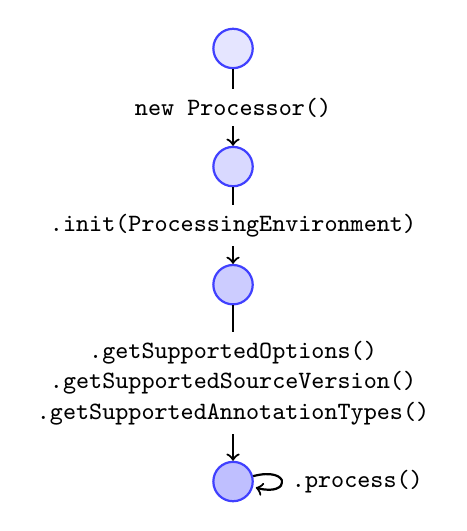
\begin{tikzpicture}
        \tikzstyle{edge-node}=[font=\small\ttfamily, align=center, fill=white]
        \tikzstyle{node}=[circle, thick, draw=black, minimum size=5mm]
        \tikzstyle{transition}=[->, thick]
        % \draw (0, -2) grid (6, 2);
        \node[node, draw=blue!75, fill=blue!10] (start) at (0, 0) {};
        \node[node, draw=blue!75, fill=blue!15] (processor) at (0, -1.5) {};
        \node[node, draw=blue!75, fill=blue!20] (processor-init) at (0, -3) {};
        \node[node, draw=blue!75, fill=blue!25] (processor-gets) at (0, -5.5) {};
        % \node[node] (process) at (0, -7.5) {};

        \draw[transition] (start) -- node[edge-node] {new Processor()} (processor);
        \draw[transition] (processor) -- node[edge-node] {.init(ProcessingEnvironment)} (processor-init);
        \draw[transition] (processor-init) -- node[edge-node] {.getSupportedOptions()\\.getSupportedSourceVersion()\\.getSupportedAnnotationTypes()} (processor-gets);
        \draw[transition] (processor-gets) edge[loop right] node[edge-node] {.process()} (processor-gets);

    \end{tikzpicture}
    \caption{Java's annotation processor lifecycle.}
    \label{fig:java-annotation-processor}
\end{figure}

\begin{listing}
    \centering
    \begin{minted}{Java}
@Retention(RetentionPolicy.RUNTIME)
@Target(ElementType.ANNOTATION_TYPE)
@interface Foo {}
    \end{minted}
    \caption{
        Example code for Java's annotation declaration.
        % Possible values for \texttt{@Retention} and \texttt{@Target} are summed up in \autoref{fig:java-annotation-class-dia}.
    }
    \label{lst:java-annotation-declaration}
\end{listing}

\begin{figure}
    \centering
    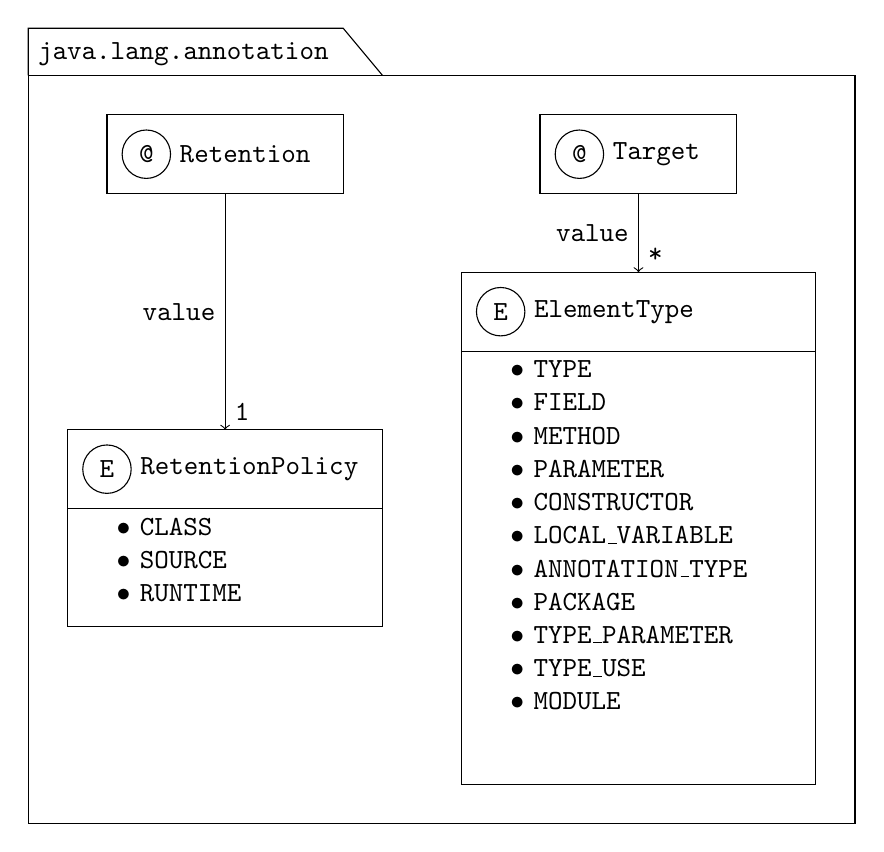
\begin{tikzpicture}
        % \draw[draw=black!20] (0, -0.5) grid (10, 10);
        \draw (0, 9) -- (0, 9.6) -- (4, 9.6) -- (4.5, 9);
        \draw (0, -0.5) rectangle (10.5, 9);
        \node[draw=none, above right] (package-name) at (0, 9) {\texttt{java.lang.annotation}};

        \node[circle, draw] (annotation-id) at (1.5, 8) {\texttt{@}};
        \node[draw=none, right=3mm] (annotation-label) at (1.5, 8) {\texttt{Retention}};
        \draw (1, 7.5) rectangle (4, 8.5);

        \node[circle, draw] (annotation-id) at (7, 8) {\texttt{@}};
        \node[draw=none, right=3mm] (annotation-label) at (7, 8) {\texttt{Target}};
        \draw (6.5, 7.5) rectangle (9, 8.5);

        \node[circle, draw] (annotation-id) at (1, 4) {\texttt{E}};
        \node[draw=none, right=3mm] (annotation-label) at (1, 4) {\texttt{RetentionPolicy}};
        \draw (0.5, 3.5) rectangle (4.5, 4.5);
        \draw (0.5, 3.5) -- (0.5, 2) -- (4.5, 2) -- (4.5, 3.5);
        \node[align=left, below right] (members) at (1, 3.5) {
            $\bullet$~\texttt{CLASS}\\
            $\bullet$~\texttt{SOURCE}\\
            $\bullet$~\texttt{RUNTIME}\\
        };

        \node[circle, draw] (annotation-id) at (6, 6) {\texttt{E}};
        \node[draw=none, right=3mm] (annotation-label) at (6, 6) {\texttt{ElementType}};
        \draw (5.5, 5.5) rectangle (10, 6.5);
        \draw (5.5, 5.5) -- (5.5, 0) -- (10, 0) -- (10, 5.5);
        \node[align=left, below right] (members) at (6, 5.5) {
            $\bullet$~\texttt{TYPE}\\
            $\bullet$~\texttt{FIELD}\\
            $\bullet$~\texttt{METHOD}\\
            $\bullet$~\texttt{PARAMETER}\\
            $\bullet$~\texttt{CONSTRUCTOR}\\
            $\bullet$~\texttt{LOCAL\_VARIABLE}\\
            $\bullet$~\texttt{ANNOTATION\_TYPE}\\
            $\bullet$~\texttt{PACKAGE}\\
            $\bullet$~\texttt{TYPE\_PARAMETER}\\
            $\bullet$~\texttt{TYPE\_USE}\\
            $\bullet$~\texttt{MODULE}\\
        };

        \draw[->] (2.5, 7.5) -- node[left] {\texttt{value}} (2.5, 4.5) node[above right] {\texttt{1}};
        \draw[->] (7.75, 7.5) -- node[left] {\texttt{value}} (7.75, 6.5) node[above right] {\texttt{*}};

    \end{tikzpicture}
    \caption{\texttt{java.lang.annotation} class diagram.}
    \label{fig:java-annotation-class-dia}
\end{figure}

\paragraph{Implementing an Annotation.}
To implement an annotation, start by declaring it as in \autoref{lst:java-annotation-declaration}.
The annotation may contain parameters that allow to add configuration when the declaration is used.
Supported types are:
\begin{compactitem}
	\item Primitive types (e.g. \keyword{int}, \keyword{long}, etc).
	\item \keyword{String}
	\item \keyword{Class<T>}
	\item \keyword{enum} types.
	\item Other annotation types.
	\item An array of the above.
\end{compactitem}
At this point the annotation is processed by the compiler but does not do anything useful.
To address that, the code needs to either handle the annotation at runtime, through reflection.
Or at compile-time, through an annotation processor.
Since processing the annotation at runtime incurs a cost, I'll only discuss the annotation processor approach.

\paragraph{Annotation Processor.}
Putting it simply, is a specific class registered at compile-time as able to process annotations.
The compiler can then make use of the class to process the new annotations.
The class itself will usually extend the \texttt{AbstractProcessor} class,
overriding some methods present in \autoref{fig:java-annotation-processor}.
The processor will then be called for each annotation belonging to the package.

Annotation processors are also able to generate code.
This is usually done by means of a library such as JavaPoet\citeurl{https://github.com/square/javapoet}.
After generation, the output code is then compiled and subject to the same treatment as handwritten files.
If the generated code, generates more code, this process repeats itself until no more code is generated.

\paragraph{Ecosystem Presence.}
Java annotations are ubiquitous.
Examples include but are not limited to the development of REST \gls{API}s,
Android applications and database tools.
As discussed in \autoref{sec:lang-preprocessors:java:annotation},
annotations are picked up by several tools and serve a plethora of purposes,
from cutting boilerplate to providing an extra layer of security and assurance.
However, being ubiquitous does not imply that resources are widely available.
Learning to develop annotations seems to be an almost exotic topic in Java,
with few quality resources available.

\subsubsection*{ExtendJ \& JastAdd}\label{sec:lang-preprocessors:java:extendj}

ExtendJ is an extensible compiler aiming at facilitating the development of Java compiler tools.
The compiler supports Java from version 5 up to 8.
The extensions are written in JastAdd \citeurl{https://jastadd.cs.lth.se/web/}{08/06/2021}, a meta-compilation system upon which ExtendJ is built.
It is possible to extend the compiler during any of the following phases: \emph{Scanning}, \emph{Parsing}, \emph{Analysis} and \emph{Code Generation}.
Extending the language with new syntax requires the modification of the \emph{Scanner} and \emph{Parser}.
The \emph{Analysis} phase occurs after parsing, when types are checked.
Hence, to extend type analysis, one must modify it in the compiler.
Finally, \emph{Code Generation} has two possible extension methods in ExtendJ:
\emph{direct bytecode generation} and \emph{desugaring}.
The latter being the simpler approach and recommended being tried before the former.
Desugaring can be used to prototype new languages constructs, by mapping them to the respective Java code.

\paragraph{Ecosystem Presence.}
While both ExtendJ and JastAdd are powerful tools, they lack of support for versions after Java 8.
Their usage is generally confined to academia being unsuited for industrial usage.
Documentation on getting up and running is also limited,
being mostly based on papers and examples rather than entry-level explanations.

\begin{listing}
    \centering
    \begin{minted}{Java}
@any Person people;
people += new Person("Bob");
people += new Person("Gene");
people += new Person("Tina");
for (Person person : people) {
    System.out.println(person.getName());
}
    \end{minted}
    \caption{
        The \texttt{@any} annotation allows an object to carry several instances of itself.
        In the example, \texttt{@any Person} is rather a collection of \texttt{Person}.
        This extension is enabled by the ExtendJ compiler.
    }
    \label{lst:jastadd-annotation-declaration}
\end{listing}

\subsection{Kotlin}\label{sec:lang-preprocessors:kotlin}

While Kotlin also allows and makes use of Java annotations, it is also possible to write plugins for the Kotlin compiler.
Compiler plugins are much more complex pieces of software in comparison with annotations,
due to the amount of detail required to take into account.
An example of such detail is the amount of Kotlin backends available, not all targeting the Java Virtual Machine.
This is also a motivation to write a compiler plugin, as annotations may not be compatible with all backends.

\subsubsection*{Kotlin Compiler Plugins}\label{sec:lang-preprocessors:kotlin:annotation}
The Kotlin compiler plugin stack is illustrated in \autoref{fig:kotlin-compiler-plugin-arch}.
From top to bottom, the first two parts are related to Gradle, the main build system for Kotlin.
These parts to not work on the plugin itself, but rather help the plugin coexist with the rest of the Kotlin ecosystem.

\paragraph{\texttt{Plugin}.}
The plugin interacts only in the Gradle segment,
it provides an entrypoint from a \texttt{build.gradle} plugin and allows plugin configuration.

\paragraph{\texttt{Subplugin}.}
The subplugin acts as the glue between Gradle and Kotlin.
It sets up a series on options for the layer below from the configuration provided in the first layer.
It also defines a plugin ID to avoid name clashing with other plugins and Maven coordinates, which allow the plugin to be downloaded.

\paragraph{\texttt{CommandLineProcessor}.}
This layer reads the arguments for \texttt{kotlinc -Xplugin}.
The options from the previous layer are passed through here.
Finally, it writes \texttt{CompilerConfigurationKeys} which will be passed to the layer bellow.

\paragraph{\texttt{ComponentRegistar}.}
This component just reads the passed keys and registers extensions to be used by the compiler.
It is possible to register several extensions at a time.

\paragraph{\texttt{Extension}.}
The extension is the main part of the plugin.
There are multiple types of extensions able to deal with the input at different levels,
from the class level to the code generation.

\paragraph{Ecosystem Presence.}
Just like the previous languages, the Kotlin compiler plugins suffer from the same discoverability problem.
While depending on it are widely used (e.g. Kotlin serialization\citeurl{https://github.com/Kotlin/kotlinx.serialization}{08/06/2021}),
the resources to learn how to develop such tools are rare.

% \begin{figure}
    \centering
    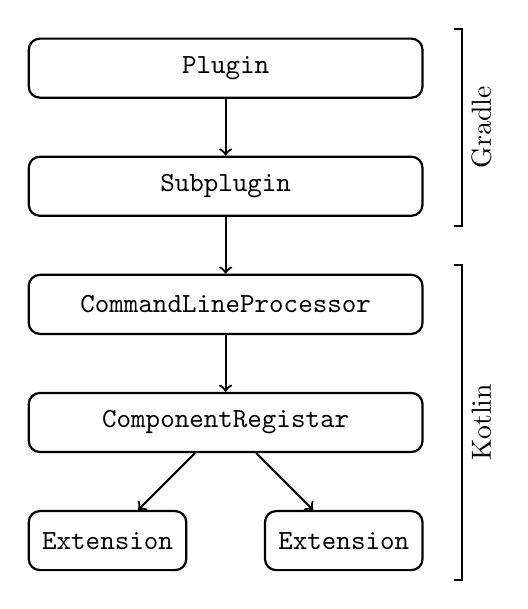
\begin{tikzpicture}
        \tikzstyle{layer}=[thick, rectangle, rounded corners, minimum height=7.5mm, minimum width=5cm, draw, font=\ttfamily]
        % \draw[draw=black!20] (-4,1) grid (4, -7);
        \node[layer] (plugin) at (0, 0) {Plugin};
        \node[layer] (subplugin) at (0, -1.5) {Subplugin};
        \node[layer] (cli-processor) at (0, -3) {CommandLineProcessor};
        \node[layer] (registar) at (0, -4.5) {ComponentRegistar};
        \node[layer, minimum width=2cm] (ext-left) at (-1.5, -6) {Extension};
        \node[layer, minimum width=2cm] (ext-right) at (1.5, -6) {Extension};

        \draw[->, thick] (plugin) -- (subplugin);
        \draw[->, thick] (subplugin) -- (cli-processor);
        \draw[->, thick] (cli-processor) -- (registar);
        \draw[->, thick] (registar) -- (ext-left);
        \draw[->, thick] (registar) -- (ext-right);

        \draw[thick] (2.9, 0.5) -- (3, 0.5) -- (3, -2) -- (2.9, -2);
        \draw[thick] (2.9, -2.5) -- (3, -2.5) -- (3, -6.5) -- (2.9, -6.5);

        \path (3, 0.5) -- node[below, rotate=90]{Gradle} (3, -2);
        \path (3, -2.5) -- node[below, rotate=90]{Kotlin} (3, -6.5);
    \end{tikzpicture}
    \caption{Kotlin compiler plugin architecture stack \autocite{Most2018}.}
    \label{fig:kotlin-compiler-plugin-arch}
\end{figure}
\begin{figure}
	\centering
	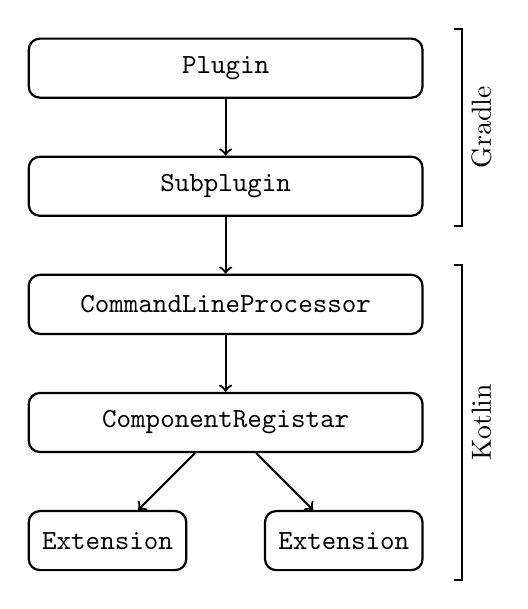
\begin{tikzpicture}
		\tikzstyle{layer}=[thick, rectangle, rounded corners, minimum height=7.5mm, minimum width=5cm, draw, font=\ttfamily]
		% \draw[draw=black!20] (-4,1) grid (4, -7);
		\node[layer] (plugin) at (0, 0) {Plugin};
		\node[layer] (subplugin) at (0, -1.5) {Subplugin};
		\node[layer] (cli-processor) at (0, -3) {CommandLineProcessor};
		\node[layer] (registar) at (0, -4.5) {ComponentRegistar};
		\node[layer, minimum width=2cm] (ext-left) at (-1.5, -6) {Extension};
		\node[layer, minimum width=2cm] (ext-right) at (1.5, -6) {Extension};

		\draw[->, thick] (plugin) -- (subplugin);
		\draw[->, thick] (subplugin) -- (cli-processor);
		\draw[->, thick] (cli-processor) -- (registar);
		\draw[->, thick] (registar) -- (ext-left);
		\draw[->, thick] (registar) -- (ext-right);

		\draw[thick] (2.9, 0.5) -- (3, 0.5) -- (3, -2) -- (2.9, -2);
		\draw[thick] (2.9, -2.5) -- (3, -2.5) -- (3, -6.5) -- (2.9, -6.5);

		\path (3, 0.5) -- node[below, rotate=90]{Gradle} (3, -2);
		\path (3, -2.5) -- node[below, rotate=90]{Kotlin} (3, -6.5);
	\end{tikzpicture}
	\caption[Kotlin compiler plugin architecture stack.]{Kotlin compiler plugin architecture stack\footnotemark.}
	\label{fig:kotlin-compiler-plugin-arch}
\end{figure}
\footnotetext{\url{https://tinyurl.com/MostK2018} (visited on 08/06/2021)}

\section{Rust Macros}\label{sec:rust-macros}

Just like C and C++, Rust offers macros as part of the language.
In essence, Rust macros are just like other languages macro's, running during compile-time to generate code.
In Rust, macros refer to a family of features (see \autoref{fig:rust-macro-family}),
\emph{declarative} macros and \emph{procedural} macros.

\begin{figure}
    \centering
    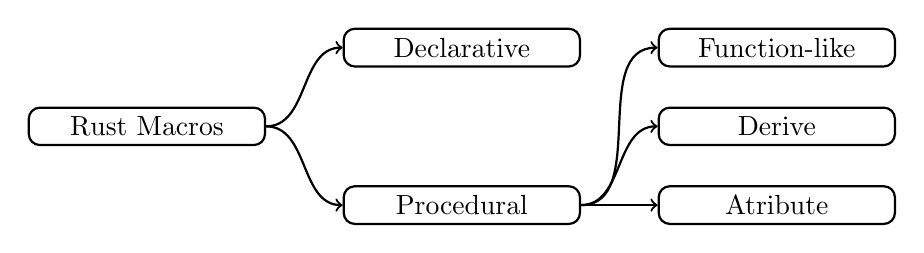
\begin{tikzpicture}
        \tikzset{
            member/.style={
                    rectangle,
                    rounded corners,
                    draw=black,
                    thick,
                    minimum width=3cm,
                },
            connection/.style={->, thick},
        }
        % \draw (0, -2) grid (6, 2);
        \node[member] (root) at (-1, 0) {Rust Macros};
        \node[member] (decl) at (3, 1) {Declarative};
        \node[member] (proc) at (3, -1) {Procedural};
        \node[member] (func) at (7, 1) {Function-like};
        \node[member] (derv) at (7, 0) {Derive};
        \node[member] (attr) at (7, -1) {Atribute};
        \draw[connection] (root) edge[out=0, in=180] (proc);
        \draw[connection] (root) edge[out=0, in=180] (decl);
        \draw[connection] (proc) edge[out=0, in=180] (func);
        \draw[connection] (proc) edge[out=0, in=180] (derv);
        \draw[connection] (proc) edge[out=0, in=180] (attr);
    \end{tikzpicture}
    \caption{Rust macro's family tree}
    \label{fig:rust-macro-family}
\end{figure}

\subsection{Declarative Macros}\label{sec:rust-macros:decl}

Declarative macros (also known as \emph{macros-by-example}) can be declared with \texttt{macro\_rules!}
and are called with function syntax (see \autoref{lst:rust-macro-rules}).

\begin{displayquote}[{\autocite[Section 3.1]{RustRef2021}}]
	Each macro by example has a name, and one or more rules.
	Each rule has two parts: a matcher, describing the syntax that it matches, and a transcriber,
	describing the syntax that will replace a successfully matched invocation.
	Both the matcher and the transcriber must be surrounded by delimiters.
	Macros can expand to expressions, statements, items
	(including traits, impls, and foreign items), types, or patterns.
\end{displayquote}

\paragraph{Transcribing.}
When a macro is invoked, the macro expander loops through the declared rules, transcribing the first successful match.
It transcribes the first successful match; if this results in an error, then future matches are not tried.
An error is thrown if the compiler cannot determine unambiguously how to parse the macro
\autocite[Section 3.1 - Transcribing]{RustRef2021}.

\paragraph{Metavariables.}
To specify a macro a user first declares a pattern which will match a given form of syntax.
\emph{Metavariables} are used to achieve such goal,
they are declared with “\texttt{\$ \keyword{name} : \keyword{fragment-specifier}}” in the macro matcher and
can match thirteen different kinds of syntax fragments \autocite[Section 3.1 - Metavariables]{RustRef2021}.
In \autoref{lst:rust-macro-rules}, the metavariable \texttt{n} is of kind \texttt{literal}
which will match literals such as \texttt{'E'}, \texttt{"Elite"} and \texttt{420} \autocite[Section 8.2.1]{RustRef2021}.

\paragraph{Repetitions} are indicated by placing the tokens to be repeated inside \texttt{\$(...)},
followed by a repetition operator, optionally with a separator token between.
This is valid both for the matcher and the transcriber.
Repetition operators are the same as the regular expression ones:
\begin{compactitem}
	\item \texttt{*} — indicates zero or more repetitions.
	\item \texttt{+} — indicates at least one repetition.
	\item \texttt{?} — indicates zero or one repetition.
\end{compactitem}

\paragraph{Hygiene} works by attaching an invisible \emph{syntactic context} to all identifiers \autocite{Wirth2021}.
Identifiers are compared over two pieces of information,
the \emph{textual value} and their \emph{syntactic context}.
The textual value consists of the variables name (e.g. \texttt{four}),
the syntactic context is a kind of scope added to variables declared inside the macro.
This is done to keep the macro declared variables from interfering with existing ones.

When expanding a declarative macro\footnotemark variables declared inside the macro belong in a different scope,
consider the macro declared in \autoref{lst:rust-macro-hygiene:declaration} and
the respective expansion in \autoref{lst:rust-macro-hygiene:expansion}.
As illustrated by \autoref{lst:rust-macro-hygiene:expansion},
line 2 is considered to be in a different context than the rest of the expanded code.
This will rightfully raise an error (shown in \autoref{lst:rust-macro-hygiene:error}),
since line's 3 \texttt{a} will not exist due to not being in the same syntactic context as line 2.

\footnotetext{
	The same mechanism does not apply to procedural macros, which are not hygienic.
	Their output will interfere with existing code if precautions are not taken \autocite{Koxiaet2020}.
}

\begin{listing}
    \centering
    \begin{minted}{Rust}
macro_rules! say_hello {
    ($n:literal) => {
        for 0..$n {
            println!("Hello, world!");
        }
    }
}
fn main() {
    say_hello!(5);
}
    \end{minted}
    \caption{Example \texttt{macro\_rules!} usage.
        When executed, the code above will print “\texttt{Hello, world!}” five times.}
    \label{lst:rust-macro-rules}
\end{listing}

\begin{listing}
    \begin{minted}{Rust}
macro_rules! using_a {
    ($e:expr) => { { let a = 42; $e } }
}
let four = using_a!(a / 10);
    \end{minted}
    \caption{
        Definition of the \texttt{using\_a} macro and usage.
        The macro simply declares a variable \texttt{a},
        set to 42 and then writes an expression which was passed in.
    }
    \label{lst:rust-macro-hygiene:declaration}
\end{listing}

\begin{listing}
    \begin{minted}[highlightlines=2,highlightcolor=blue!10]{Rust}
let four = {
    let a = 42;
    a / 10
};
    \end{minted}
    \caption{
        \autoref{lst:rust-macro-hygiene:declaration} line 9's macro expansion.
        Declarations with a blue background will be placed in a different \emph{scope} than the others,
        thus the \texttt{a} for lines 2 and 3 will not be considered the same.
    }
    \label{lst:rust-macro-hygiene:expansion}
\end{listing}

\begin{listing}
    \begin{minted}{text}
error[E0425]: cannot find value `a` in this scope
  --> src/main.rs:13:21
   |
   | let four = using_a!(a / 10);
   |                     ^ not found in this scope
    \end{minted}
    \caption{
        The expansion in \autoref{lst:rust-macro-hygiene:expansion} will result in an error during compile-time
        since the \texttt{a}s in line 2 and 3 are considered to belong to different contexts.
    }
    \label{lst:rust-macro-hygiene:error}
\end{listing}


\subsection{Procedural Macros}\label{sec:rust-macros:proc}
Rust also has another macro mechanism, \emph{procedural macros},
these can take three forms: \emph{function-like macros}, \emph{derive macros} and \emph{attribute macros}.
In a nutshell, procedural macros allow users to run code at compile time, consuming and producing Rust syntax.

\subsubsection*{Function-like Macros}
Function-like macros and declarative macros are similar regarding invocation, being indistinguishable from each other,
and output, completely replacing the original call.
However, the similarities stop there as their implementation methods are completely different.

\paragraph{Definition.}
Function-like macros are defined by a public function with the \texttt{proc\_macro} attribute and
a signature of type \texttt{(TokenStream) -> TokenStream}.
Everything contained inside the call delimeters of the macro invocation is input to the function,
as previously referred, the output will completely replace the macro call.

\paragraph{Domain Specific Languages.}
While the macros discussed next also provide their contribution for domain specific languages in Rust,
function-like macros provide the necessary tools to write an embedded DSL.
The Rust ecosystem developers have developed HTML DSLs\citeurl{https://github.com/lambda-fairy/maud}{08/06/2021}$^,$\citeurl{https://github.com/bodil/typed-html}{08/06/2021}
(see the example in \autoref{lst:rust-html-dsl}) and
the possibility to run Python inside Rust\citeurl{https://github.com/fusion-engineering/inline-python}{08/06/2021}.

% \begin{listing}
    \begin{minted}{Rust}
html! {
    h1 { "Hello, world!" }
    p.intro {
        "This is an example of the "
        a href="https://github.com/lambda-fairy/maud" { "Maud" }
        " template language."
    }
}
    \end{minted}
    \caption{HTML DSL embedded in Rust. Example taken from \autocite{Wong2021}.}
    \label{lst:rust-html-dsl}
\end{listing}
\begin{listing}
    \begin{minted}{Rust}
html! {
    h1 { "Hello, world!" }
    p.intro {
        "This is an example of the "
        a href="https://github.com/lambda-fairy/maud" { "Maud" }
        " template language."
    }
}
    \end{minted}
    \caption[HTML DSL embedded in Rust.]{HTML DSL embedded in Rust.\footnotemark}
    \label{lst:rust-html-dsl}
\end{listing}
\footnotetext{\url{https://github.com/lambda-fairy/maud} (visited in 08/06/2021)}

\subsubsection*{Derive Macros}\label{sec:rust-macros:proc:derive}
Derive macros likely are the most common kind of procedural macro in Rust,
they are usually used to \emph{derive} a \keyword{trait} implementation from a \keyword{struct} (see \autoref{lst:rust-derive-debug}).
They define new inputs for the \texttt{derive} attribute,
and can also create new items given the token stream of a \keyword{struct}, \keyword{enum} or \keyword{union}.

\paragraph{Definition.}
Just like function-like macros,
derive macros are defined as a public function with the \texttt{proc\_macro\_derive} attribute
and a signature of \texttt{(TokenStream) -> TokenStream}.
The input is a token stream of the item with the \texttt{derive} attribute,
the output is a set of items that are appended to the module or block where the input token stream is in.
In \autoref{lst:rust-derive-debug} the \keyword{Debug} implementation will be appended to the end of the structure.

\paragraph{Helper Attributes.}
Derive macros are also able to add additional attributes to the scope of the current item.
Such attributes are called \emph{derive macro helper attributes} and they are \emph{inert},
that is, they are not processed by themselves but rather serve as annotations (see \autoref{lst:rust-derive-error}).

\begin{listing}
    \centering
    \begin{minted}{Rust}
#[derive(Debug)]
struct Coordinate {
    x: f32,
    y: f32,
    x: f32,
}
    \end{minted}
    \caption{
    Example usage of \ttt{\textcolor{attrgreen}{\#[derive(...)]}},
    in this case deriving \keyword{Debug} enables the structure to be printed with
    “\mintinline{Rust}{println!("{:?}", coord)}”.
    }
    \label{lst:rust-derive-debug}
\end{listing}

\begin{listing}
    \centering
    \begin{minted}{Rust}
#[derive(Error)]
enum CoordinateError {
    #[error("Invalid coordinates {0}")]
    InvalidCoordinates(Coordinates),
}
    \end{minted}
    \caption{
        Example usage of a derive macro with helper attributes,
        in this case the \texttt{error(...)} defines an error message with a \texttt{Coordinates} parameter.
    }
    \label{lst:rust-derive-error}
\end{listing}

\subsubsection*{Attribute Macros}\label{sec:rust-macros:proc:attr}
Attribute macros define new outer attributes,
in contrast to the attributes discussed in \autoref{sec:rust-macros:proc:derive},
attribute macros are processed as independent units and not as an annotation.
They can be attached to items (see \autocite[Section 6]{RustRef2021}),
including items in \keyword{extern} blocks, inherent and trait implementations, and trait definitions.

\paragraph{Definition.}
Like the other macros, attribute macros are also declared by a public function with the \texttt{proc\_macro\_attribute},
however, their function signature takes two parameters instead of one, being \texttt{(TokenStream, TokenStream) -> TokenStream}.

The first parameter is the token tree following the attribute name, for example, in \autoref{lst:rust-rocket-attr}
it would contain the token tree of \texttt{("/hello/<name>/<age>")},
in the case the attribute is written as a bare attribute name (e.g. \texttt{\#[attribute]}),
the token tree is empty.

The second parameter is the token tree of the item the macro is attached to,
the function output will \emph{replace} such item with the return item or items.

While attribute macros are able to replace the input stream,
they can also leave the stream unchanged and check for code properties (e.g. if all variables start with a given prefix).

\begin{listing}
    \centering
    \begin{minted}{Rust}
#[get("/hello/<name>/<age>")]
fn hello(name: String, age: u8) -> String {
    format!("Hello, {} year old named {}!", age, name)
}
    \end{minted}
    \caption{
        Attribute macros are commonly used in web frameworks to provide an easy way to declare an endpoint.
        In this example (taken from \autocite{Rocket2021}) the user declares that \texttt{GET} requests to \texttt{hello/}
        have two path parameters (\texttt{name} and \texttt{age}) and should be handled by the \texttt{hello} function.
    }
    \label{lst:rust-rocket-attr}
\end{listing}

\begin{table}
	\centering
	\begin{tabular}{l|l|l|l}
		Macro Type    & Input Processing & Output Processing & Invocation                 \\
		\hline
		Declarative   & Pattern Matching & Replace           & \texttt{macro!}            \\
		Function-like & User programmed  & Replace           & \texttt{macro!}            \\
		Derive        & User programmed  & Append            & \texttt{\#{[}derive(...)]} \\
		Attribute     & User programmed  & Replace           & \texttt{\#{[}attribute]}
	\end{tabular}
	\caption{Rust macros properties summary.}
	\label{tab:rust-macros}
\end{table}

\subsection{Summary}
In summary, Rust enables metaprogramming through macros, the same can be divided into two categories,
declarative macros, with work through pattern matching, and procedural macros.
Their main characteristics are summarized in \autoref{tab:rust-macros}.

Declarative macros (\autoref{sec:rust-macros:decl}) work mainly through pattern matching,
they are the best tool to avoid code repetition without putting in the effort of writing a token parsing macro.
However, for more complex tasks, declarative macro's readability quickly degrades leading to an unpleasant developing experience.

Procedural macros (\autoref{sec:rust-macros:proc}) can be further subdivided into three categories,
being \emph{function-like}, \emph{derive} and \emph{attribute} macros.
Function-like macros can be considered as an alternative to declarative ones,
they allow for more functionality and flexibility being possible for the code behind them
to be replaced from one to the other without changes on the user's part.
In comparison with other procedural macros, function-like macros allow for the creation of an embedded DSL inside Rust while the others are mainly annotations.
Derive macros are mainly used to extend existing structures with traits that can be derived automatically (e.g. \keyword{Debug}).
Finally, attribute macros can be used to modify existing code or simply check for code properties (e.g. if an \keyword{enum} fields are sorted).

\section{Approaches to Behavioral Types}\label{sec:behavioral-approaches}

As previously discussed, there are several kinds of approaches to behavioral types,
some aim to bridge modern languages and behavioral types,
others build a language from scratch.
Building a new language is a more attractive approach since there is no requirement for retrofitting.
This approach is more common in the typestate domain, with Vault and Plaid being prime examples.
The library approach receives more attention from the session types domain,
where projects aim to implement them in existing languages such as Java, Go and Rust.

\subsection{Session Types}
As established so far, session types are mostly used for communication protocols,
defining message types and their order in a conversation.
Session types also share common ground with typestates as works StMungo \autocite{Dardha2017, Kouzapas2018, Voinea2020}
and others \autocite{Gay2015, Vasconcelos2017} demonstrate.

\paragraph{StMungo} it is a transpiler from Scribble \autocite{Yoshida2014} to Java based on session types and typestate.
The transpilation process takes Scribble local protocols as input, generating Mungo typestate specifications and Java skeleton implementation code.
The output is then checked by Mungo \autocite{Dardha2017, Kouzapas2018, Voinea2020}.
This process is based on a formal translation of session types into typestate specifications for channel objects, and
extends the translation from binary to multiparty session types.

\paragraph{A Session Type Provider.}
The work by Neykova et al. \autocite{Neykova2018} leverages F\#'s type providers to provide developers with practical session types along with refinements.
The refinements enable the placement of constraints regarding the protocol's messages,
these are described using Scribble \autocite{Yoshida2014} along with the rest of the protocol;
the protocol and its respective refinements are validated and the .NET platform generates the required code for the F\# \gls{API}s.

Furthermore, this approach allows users to still use features like autocomplete
(something that is still being worked in Rust's ecosystem) and documentation.
As one can expect, this approach also reduces bugs and simplified several error-prone parts of development.

\paragraph{Session Types for Rust.}
As far as I am aware, the work on Rust session types was started by Jespersen et al. \autocite{Jespersen2015},
such work was limited as it only supported binary session types.
It builds on a Haskell-based approach \autocite{Pucella2008}, mirroring the implementation interface.

The type constructs in the original session types formulation have correspondents in the Rust implementation,
this is part of a DSL embedded in the Rust type system.
The library makes use of \keyword{unsafe} to allow for transmutation (i.e. unsafe type casting)
and sending untyped values over the channels.

Finally, the library is able to provide compile-time safety, that is,
the code will not compile if the channel's protocols do not match.

\paragraph{The \texttt{sesh}} crate \cite{Kokke2019}, in contrast to \texttt{session-types} \autocite{Jespersen2015},
builds on a different theory, provides much cleaner types and embraces Rust's affine type system,
instead of actively trying to make it linear.
While the crate requires no use of \texttt{unsafe}, it does require a \emph{nightly} compiler,
unsuited for production environments.

Like \texttt{session-types}, the \texttt{sesh} crate provides the required abstractions to use session types in Rust,
however, the crate's documentation is limited, possibly being \quotes{inaccessible} to less experienced users
w.r.t. Rust and session types.

\paragraph{Multiparty Session Types for Rust.}
Work on multiparty session types started with Lagaillardie et al. \autocite{Lagaillardie2020}.
This work makes use of the Scribble \autocite{Yoshida2014} toolchain, just like StMungo;
and it is a thin wrapper over previous work done by Kokke \autocite{Kokke2019}.
Similarly to the previously presented work \autocite{Jespersen2015},
this work also takes advantage Rust's type system to provide compile-time safety.
While using Scribble allows the library to make use of a tried and tested toolchain,
it also implies the usage of an external tool, which in previous works was not necessary \autocite{Jespersen2015, Kokke2019}.

\paragraph{Rumpsteak} \autocite{Cutner2021} is a Rust library targeting asynchronous applications using \texttt{async}/\texttt{await},
it offers clean session types and its approach relies heavily on macros.
The crate works by defining a global type which is projected into roles,
this is done by Scribble which in turn requires an external toolchain\citeurl{https://github.com/nuscr/nuscr}{08/06/2021};
from each role an endpoint finite state machine is extracted and optimized,
in the end an \gls{API} is generated which can then be used to build each process.

To enforce linear resource usage when build the processes
the library makes use of the type system to enforce the consumption of each \quotes{state};
enforcing protocol completion is done through a closure,
which takes the initial session type and returns a terminal \texttt{End} type,
a session is then required to be run until completion otherwise the return type will not be respected and the type checker will complain.

\subsection{Typestate}
In the work of Ancona et al. \autocite[Section 2.3]{Ancona2016} several approaches to typestates are enumerated.
While most approaches create a new language,
approaches like Fugue \autocite{DeLine2004} simply build on top of existing languages.
This kind of approach is extremely valuable as it bridges the gap between existing programming languages and the theoretical field.

\paragraph{Vault} is a programming language with the aim of researching lifetime tracking and the symbolic state of objects \autocite{Fahndrich2002}.
Vault introduces two new concepts — \emph{adoption} and \emph{focus}, which serve to relax constrains imposed by a linear type system.
Since aliasing can be controlled through the linear type system, Vault is able to check for states, hence supporting typestate.
Vault bridges the best of both worlds by splitting programs into two groups:
the ones able to be checked for protocols (i.e. \emph{typestated}) and
the ones free of aliasing restrictions and thus unable to verify protocol rules.

The adoption mechanism works by means of an \emph{adopter} (i.e. which adopts a linear reference) and an \emph{adoptee} (i.e. the adopted reference).
Through adoption, the adopted linear reference is consumed, and thus cannot be directly accessed.
Furthermore, the lifetime of each reference alias is tied to the lifetime of the adopter.
When the adopter is freed, all adopted references recover their linear type.

The focusing mechanism provides a temporarily linear view on a nonlinear object.
The focused object is required to be live and of the same type in the end of the focus usage.
Access to the parent of the focused object is temporarily revoked, disabling alias access.

\paragraph{Fugue} is a software checker that enables interface protocols (i.e. typestates) to be specified as annotations \autocite{DeLine2004}.
It provides two main protocol checking functions, \emph{resource protocols} and \emph{state-machine protocols}.
Resource protocols relate to the allocation and release of resources,
since Rust takes care of such concerns through ownership I will not discuss this feature of Fugue.

State-machine protocols allow the programmer to constrain the sequence of method calls on an object.
This is also known as typestate, as one can only transition between valid states.
In Fugue, the developer adds annotations to the object's methods and from them, a state-machine is derived.
Fugue also allows for states to relate to one another.
Consider the example in \autoref{lst:csharp-fugue-states}; by relating the states in the \texttt{OuterSocket} class
with the \texttt{innerSocket} field states Fugue can ensure that \texttt{OuterSocket} is a well-behaved client of the field's class.

\begin{listing}
    \centering
    \begin{minted}{csharp}
[WithProtocol("open", "closed")]
class OuterSocket {
    [InState(”connected”, WhenEnclosingState=”open”),
        NotAliased(WhenEnclosingState=”open”)]
    [Unavailable(WhenEnclosingState=”closed”)]
    private Socket innerSocket;
}
    \end{minted}
    \caption{
        Relating a class's states with the \texttt{innerSocket} states.
        In this example, the \texttt{OuterSocket}'s \texttt{open} state is related with the \texttt{connected} state of the socket.
        This ensures that the \texttt{OuterSocket} is a well-behaved client of \texttt{innerSocket}.
    }
    \label{lst:csharp-fugue-states}
\end{listing}

\paragraph{Plaid} is a typestate-oriented language.
The idea, proposed in \autocite{Aldrich2009}, is based on support for first-class typestates in an object-oriented setting.
In Plaid, objects are described by their state rather than members.
While the object is able to have fields common to all states, there is also the possibility for fields to be exclusive to a given state.
For the example of the \texttt{File} which can be either in the \keyword{Open} state or the \keyword{closed}, the former state would have an OS file descriptor,
while the closed state would not. The path to the file could be available for both states, since it would allow the file to be re-opened.

In Plaid, methods can make the object transition between states. Building on the file example,
the method \texttt{open} would transition the file from the \keyword{Closed} state to the \keyword{Open} state.
Plaid also introduces a series of aliasing control keywords,
\keyword{unique} disallows aliasing on an object while allowing for state transitions,
\keyword{immutable} disallows mutation (i.e. state transitions),
\keyword{shared} makes an object behave like it normally would in Java,
allowing aliasing (since it allows aliasing, it also requires runtime checks over state on sensitive operations).

\paragraph{Mungo} is a static analysis tool \autocite{Dardha2017, Kouzapas2018, Voinea2020} for Java programs.
It checks typestate properties and can be divided into two components, a Java-like language to define typestate specifications
and a typechecker, which checks that objects follow the typestate specification.
Specifications are written as separate files and can then be used in Java classes through annotations, as demonstrated in \autoref{lst:java-mungo-typestate}.
The annotations enable Mungo to be unobtrusive in projects since annotations are not required to be processed (as seen in \autoref{sec:lang-preprocessors:java:annotation}).
\begin{displayquote}[{\autocite[Section 1.2]{Dardha2017}}]
	If a class has a typestate specification, the Mungo typechecker analyses each object of that class in the program and extracts the method call behaviour (sequences of method calls) through
	the object’s life. Finally, it checks the extracted information against the sequences of method calls allowed by the typestate specification.
\end{displayquote}

\begin{listing}
    \centering
    \begin{minted}[linenos=false]{csharp}
@Typestate("StateIteratorProtocol")
class StateIterator { /* ... */ }
    \end{minted}
    \caption{
        Mungo's \texttt{Typestate} annotation. Normal Java code ends up ignoring the annotation.
        However, Mungo is able to process it and check the class calls against the specification to ensure typestate compliance.
        In this case the class specification is \texttt{StateIteratorProtocol}.
    }
    \label{lst:java-mungo-typestate}
\end{listing}

\subsection{Summary}

In summary, behavioral types is a topic which for now, is still mostly confined to the academia circles.
Despite the efforts put into the development of tools for “\emph{business}” languages,
the tools were either abandoned (e.g. Fugue) or
superseded by other developments in the field (e.g. the initial work in session types for Rust).
Languages developed for research purposes (e.g. Vault and Plaid) seem to make little to no effect on the outside world.
While adoption of the language itself is not expected, such could be expected for the mechanisms,
though it does not seem to be the case.
Finally, in the case of tools (e.g. Scribble and Mungo), they seem to pick the most traction from academia.
The motivation seems to be based on the possibility of extension and continuous improvement.
However, they seem to suffer the same destiny as others, causing little to no impact in the outside world.